%!TEX root = ../swiatlow_thesis.tex
\label{chapter:sm}

The Standard Model (SM) of particle physics is the enormously successful set of theories, developed mostly in the 1960s-1970s, which are the best known description of fundamental physics. The SM describes all known matter and all known forces and interactions with startling precision: some observables, such as the value of the electromagnetic coupling constant, $\alpha$, have even been measured to within 1 part in $10^{10}$ of their predicted value \editnote{cite}. Moreover, many precision analyses performed in a huge variety of final states at the LHC, summarized in Figure~\ref{fig:sm:summary}, all show strong agreement with the prediction: the SM has been extraordinarily successful at describing the high-energy physics frontier.

%%%%%%%%%%%%%%%%

\begin{figure}
\centering
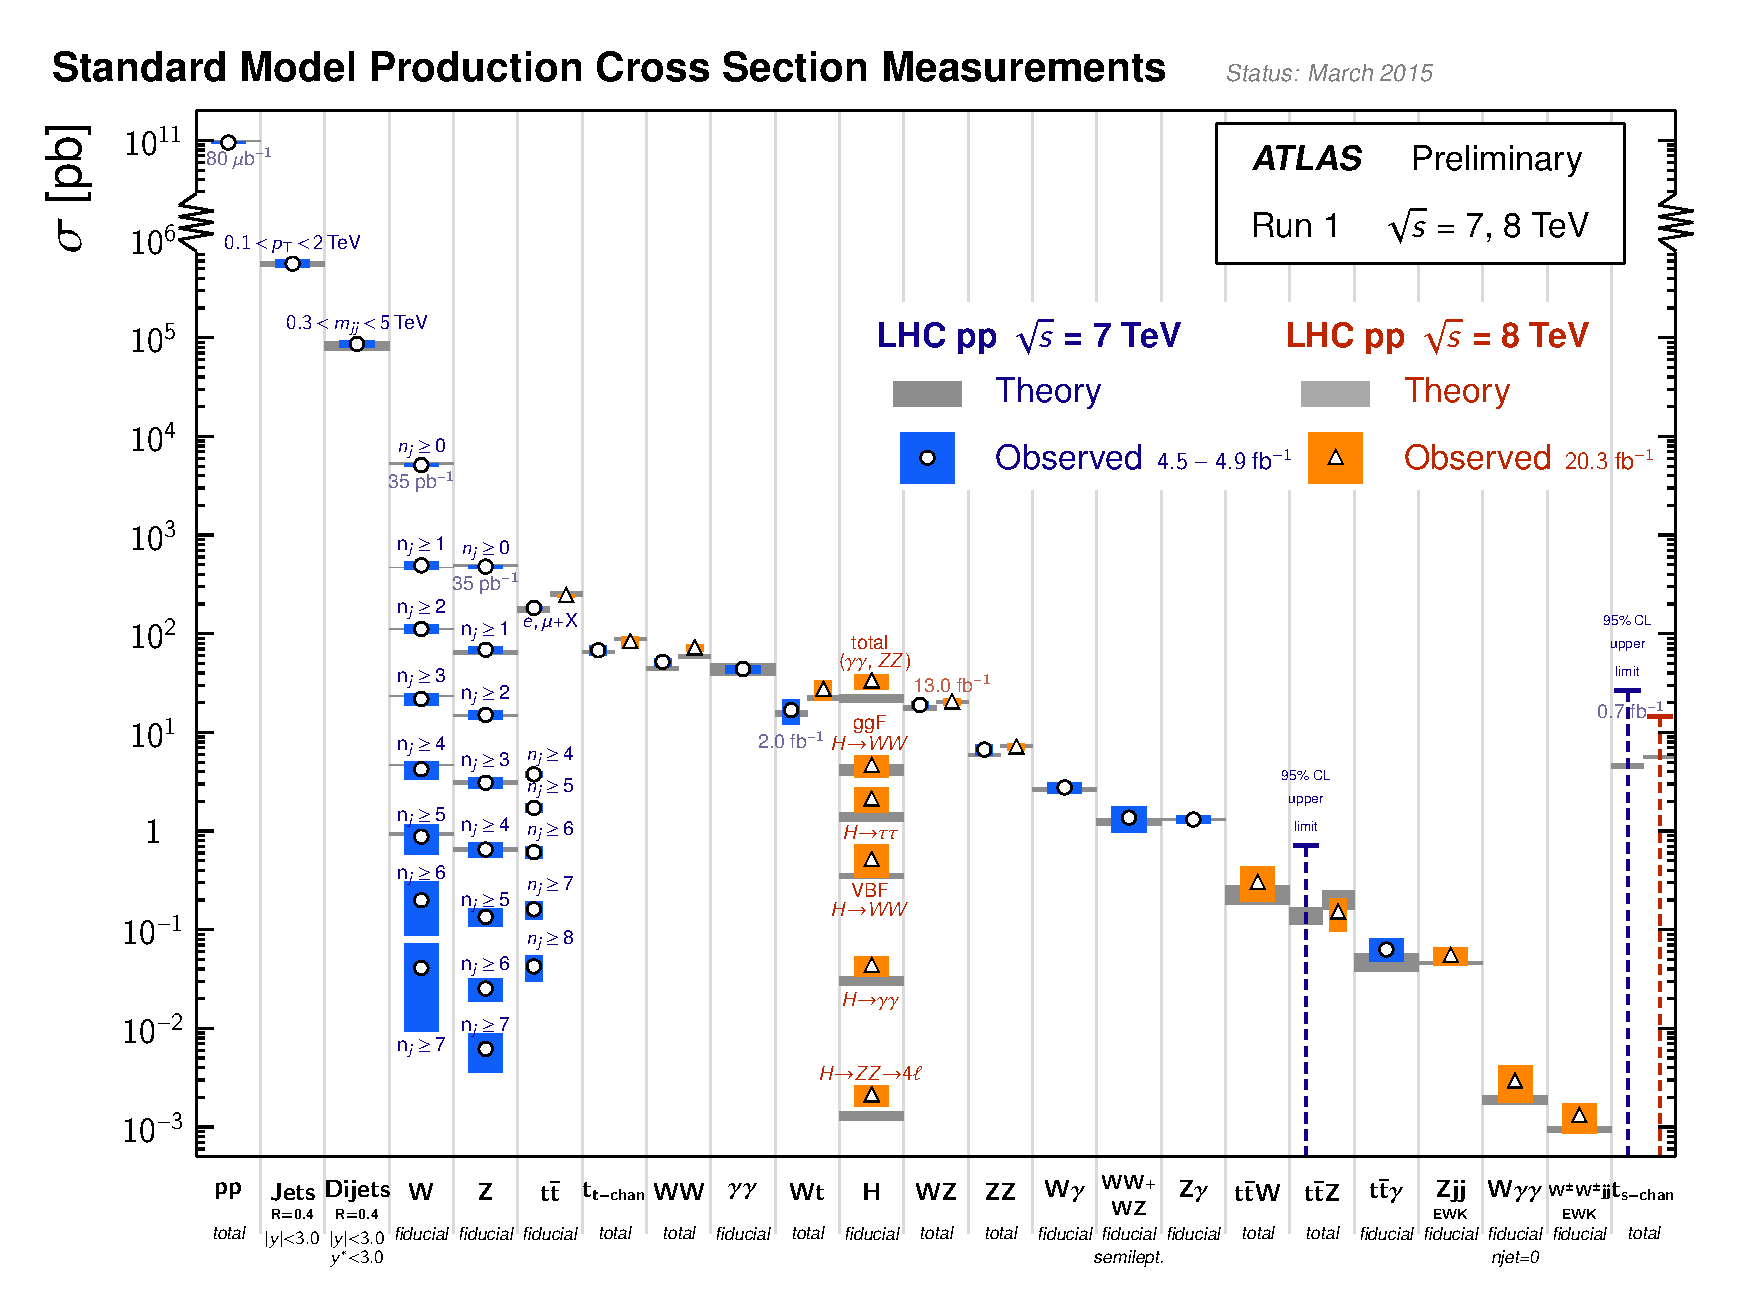
\includegraphics[width=0.7\textwidth]{summary.pdf}
\label{fig:sm:summary}
\caption{Summary of SM cross-section measurements performed in ATLAS, showing the theoretical prediction and the observed value. The agreement across all the various channels is striking.}
\end{figure}

%%%%%%%%%%%%%%%% 

The theory consists of two main parts: the Glashow-Weinberg-Salam theory of electroweak interactions, which describes the electromagnetic and weak nuclear forces, and Quantum Chromodynamics, which describes the strong nuclear force. Together these form the symmetry group of the Standard Model, $SU(3)_C \otimes SU(2)_W \otimes U(1)_Y$. With the discovery of the Higgs Boson, the mechanism of symmetry breaking in the electroweak sector has been elucidated, and all the particles predicted by the model have been identified. While the SM is complete in this sense, there are still many questions which it does not address, and some of these will be addressed in Chapter~\ref{chapter:susy} and \ref{chapter:search}. At the same time, some predictions of the SM-- the decay channels of the Higgs Boson, or the details of parton showering in QCD-- are still not fully understood, and one new measurement of such SM phenomena is presented in Chapter~\ref{chapter:color}.

The following sections give an overview of the SM and outline some of its most powerful successes. The approach will be very cursory, aiming to give a broad overview of the SM Lagrangian and how various parts of it function; detailed references can be found in \ldots. \editnote{Citations on main historial papers?}



\section{The Electroweak Force and Spontaneous Symmetry Breaking}

\editnote{How do I cite Schwartz?}

To start, it is interesting to characterize the electroweak force, i.e. the $SU(2)_W \otimes U(1)_Y$ part of the SM. Note that the $U(1)_Y$ is the gauge group of \textit{hypercharge}, not the low-energy $U(1)$ associated with electromagnetism. Similarly, the particles associated with the $SU(2)_W$ are not the vector bosons $W$ and $Z$: instead, linear combinations of all these fields form the familiar mass eigenstates. 

The Lagrangian of the electroweak sector (writing down all renormalizable and gauge-invariant terms), is:
%
\begin{equation}
\label{eqn:sm:electroweak_l}
\mL = - \frac{1}{4} (W_{\mu\nu}^a)^2 - \frac{1}{4} B_{\mu\nu}^2 + (D_\mu H)^\dagger (D_\mu H) + m^2 H^\dagger H - \lambda(H^\dagger H)^2,
\end{equation}
%,
where $W_\mu^a$ are the $SU(2)$ gauge bosons, $B_\mu$ is the hypercharge gauge boson (and $B_{\mu\nu} = \partial_\mu B_\nu - \partial_\nu B_\mu$), and $H$ is a complex doublet with hypercharge $1/2$, called the Higgs multiplet. The covariant derivative $D_\mu$ is defined as:
%
\begin{equation}
D_\mu H = \partial_\mu H - i g W_\mu^a \tau^a H - \frac{1}{2} i g' B_\mu H,
\end{equation}
%
with $g$ and $g'$ as the $SU(2)$ and $U(1)$ coupling constants, and $\tau^a$ as the standard $SU(2)$ generator. The last part of the Lagrangian, $V(H) = -m^2 |H|^2 +\lambda |H|^4$, is the \textit{Higgs potential}. A potential of this form has a minimum at $|\langle H \rangle| = \sqrt{\frac{2 m^2}{\lambda}}$, which induces a vacuum expectation value (vev) in the potential. This vev means that the ground state spontaneously breaks the symmetry of the potential. Written out in terms of the multiplet, and taken as real and in one direction only without loss of generality, this vev can be written as:
%
\begin{equation}
H = \exp \left( 2i \frac{\pi^a \tau^a}{v} \right) \colvec{2}{0}{\frac{v}{\sqrt{2}}+ \frac{h}{\sqrt{2}}}
\end{equation}
%
where $v = m / \sqrt{\lambda}$, and $h$ is a real scalar field. The choice of unitary gauge allows us to set $\pi = 0$, simplifying the phase of the vev. Plugging this into the covariant derivative term, and ignoring $h$ terms for now, we have:
%
\begin{equation}
|D_\mu H|^2 = g^2 \frac{v^2}{8} \left[ (W_\mu^1)^2 + (W_\mu^2)^2 + \left( \frac{g'}{g} B_\mu - W_\mu^3 \right) \right]
\end{equation}
%
These are the mass terms of the three massive gauge bosons (each proportional go $\frac{g^2 v^2}{8}$). To simplify these masses, we introduce $\tan(\theta_w) = \frac{g'}{g}$, which allows us to write:
%
\begin{align}
Z_\mu &\equiv \cos \theta_w W_\mu^3 - \sin \theta_w B_\mu\\
A_\mu &\equiv \sin \theta_w W_\mu^3 + \cos \theta_w B_\mu
\end{align}
%
and introduce a change of linear basis for the $W^{1,2}$ terms as $W_\mu^{\pm} \equiv \frac{1}{\sqrt{2}} (W_\mu^1 \mp i W_\mu^2)^2$. Plugging this into the original mass terms, we get:
%
\begin{align}
m_A &= 0\\
m_W &= \frac{v}{2} g\\
m_Z &= \frac{v}{2} \sqrt{g^2 +g'^2} = \frac{m_W}{\cos \theta_w}
\end{align}
%
These are the mass terms of the familiar photon, $W$, and $Z$ bosons. The original Lagrangian in Equation~\ref{eqn:sm:electroweak_l} contained only massless bosons: in fact, writing down masses directly would break the $U(1)$ invariance of the Lagrangian. \editnote{More on this?} Instead, the breaking of the symmetry of the Higgs potential with the vev has given various linear combinations of the initially massless bosons masses, which originate as three out of the four original degrees of freedom of the complex Higgs doublet. 

Using these transformations on the rest of the original Lagrangian allows for the derivation of the kinetic terms of each boson, as well as the interactions (which are considerably more complicated now that we have broken the original electroweak symmetry). Returning now to the previously ignored $h$ term, we can collect its kinetic terms and couplings to get:
%
\begin{equation}
\mathcal{L}_\mathrm{Higgs} = - \frac{1}{2} h \left(\square + \frac{2\lambda}{v^2}\right) h + \mathrm{interactions}.
\end{equation}
%
These are the kinetic and (tree-level) mass terms of a new scalar particle, the Goldstone boson associated with the vev spontaneously breaking the electroweak symmetry, and the last degree of freedom of the original complex Higgs multiplet. This Higgs boson, discovered by the ATLAS and CMS collaborations on July 4, 2012, was the ``last piece'' of the Standard Model, and its discovery confirmed one of the final open questions of the SM. That is not to say that there are no remaining puzzles, and indeed, Section~\ref{chapter:susy:problems} will address some that are directly related to the Higgs.

\section{Quantum Chromodynamics and Strong Interactions}

%define QCD lagrangian, discuss renormalization at high level, sign of beta function leading to asymptotic freedom
Next, we characterize the Quantum Chromodynamic (QCD) force, which is governed by the symmetry group $SU(3)_C$. The QCD Lagrangian, once again defined by writing down all renormalizable and gauage invariant terms, is defined as:
%
\begin{equation}
\mL_{\mathrm{QCD}} = \sum_f i \bar{\psi_f} D_\mu \gamma^\mu \psi_f - \frac{1}{4} G_{\mu\nu}^a G_{a}^{\mu\nu}.
\end{equation}
%
where the covariant derivative is defined as:
%
\begin{equation}
D_\mu = \partial_\mu - i g_s G_\mu^a T^a
\end{equation}
%
The sum is over the $f$ families of the quarks, $\psi_f$, which will be described in more detail in Section~\ref{chapter:sm:matter}; $g_s$ is the strong coupling constant, $G_\mu^a$ are gluon fields, and $T^a$ are the generators of the $SU(3)$ group. $G_{\mu\nu}^a$, like the $B_{\mu\nu}$ terms from the electroweak interaction, is a field strength, defined as:
%
\begin{equation}
G_{\mu\nu}^a \equiv \partial_\mu G_\nu^a - g_s f^{abc}G_\mu^b G_\nu^c
\end{equation}
%
where $f^{abc}$ are the $SU(3)$ structure constants. The first term in the Lagrangian clearly provides the kinetic term for the quarks, and their interactions with gluons; the second term, when expanded, provides the kinetic term for gluons and their self-interactions, which include terms with both 3-gluon vertices and 4-gluon vertices. Note the Lagrangian has been written with the color index suppressed: the $\psi$ are in reality column vectors over $\alpha$, the color index, and the $G$ term is a matrix, with two color indices $\alpha, \beta$. This unique color charge of quarks and gluons, typically identified as red, blue, and green, gives rise to a number of interesting phenomena. For example, the three quarks are essentially independent particles, explaining why decays of particles such as the $Z$-boson are more prevalent to quarks (as decays occur equally to all types, and the additional color factor means there are more types of quarks).

\subsection{Asymptotic Freedom}

The quantization of the QCD Lagrangian (or really, any field theory) allows for so-called \textit{loop terms}, such as Figure~\ref{fig:sm:loop}, to appear in calculations. These loops, which appear as perturbative corrections for many processes, are formally infinite as the momentum in the loop is integrated over all possible momentums and grows without bound. The solution is a technique referred to as \textit{renormalization}, which deforms the theory in such a way as to keep the solutions finite. Several renormalization schemes-- which all give the same results-- exist, and they can all be thought of as setting some scale which cuts off the infinite integrals in the loops, or which absorb the ``bad,'' un-physical, infinite part of an integral and leave a physical result. The loops then become finite corrections to various properties of the theory-- masses, coupling constants, and so forth-- accurate to some order of the perturbative expansion.

%%%%%%%%%%%%%%%%

\begin{figure}
\centering
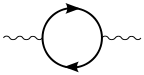
\includegraphics[width=0.25\textwidth]{loop.png}
\label{fig:sm:loop}
\caption{An example of a loop, whose contribution to a matrix element is formally infinite, in a QFT calculation.}
\end{figure}

%%%%%%%%%%%%%%%% 

One particularly interesting set of corrections is for the coupling constant, $g_s$ for the strong force\footnote{$g$ and $g'$ for the electroweak force also receive such a correction, but for reasons that will be explained, this correction is not as important for the electroweak force.} The correction to the coupling constant is parameterized by the $\beta$-function, which is used as a part of the \textit{renormalization group equation} to characterize the evolution of the coupling as a function of the $\mu/\Lambda$, or the energy scale over the cut-off of the theory. A positive value of the $\beta$-function implies that the strength of the coupling grows with energy-- this is the direction of the evolution of the electroweak couplings, for instance\footnote{In particular, the $\beta$-function is the coefficient of a $\ln{\mu/\Lambda}$ term in the RGE equation which determines the strength of the coupling constant $g$. So the sign of the $\beta$-function determines whether the RGE is a growing or shrinking exponential, to first order.}. The $\beta$-function for QCD, on the other hand, is:
%
\begin{equation}
\beta(\alpha_s) = - \frac{\alpha_s^2}{2\pi} \left(11 - \frac{4}{3}n_\mathrm{colors}\right)
\end{equation} 
%
where $\alpha_s = g_s^2 / 4\pi$. The terms here arise from a particularly long calculation (see \ldots), but can be understood to arise from the gluonic self-interactions. Since in the SM QCD $n_\mathrm{colors} = 3$, this is negative: the strength of QCD shrinks as the energy scale increases. This phenomena is referred to as \textit{asymptotic freedom}: as the energy scale $\mu$ approaches infinity, the strength of the force drops to zero. Conversely, at low energies, the coupling constant approaches infinity-- meaning that the perturbative expansion used to derive this breaks down, and a new approach must be taken. 

\subsection{Confinement}

The non-perturbative evolution of $g_s$ at low $\mu$ suggests that a transition occurs in the theory: in fact, this is the process of \textit{color confinement}. Confinement means that objects which are charged under the strong force-- quarks and gluons-- will form bound states with neutral color, such that direct color is never observed. Free quarks and gluons, produced in collisions or decays of other particles, will use some of their energy to create partners to form neutral combinations. This process is also referred to as \textit{hadronization}, in that it is the transition of the partons of QCD into the stable (or semi-stable) hadrons (either mesons, composed of two quarks, or hadrons, composed of three quarks) which are observable in experiment. 

This process has an incredible impact on the experimental accessibility of strongly interacting particles: in particular, it means that such particles are never directly observable, but will only ever be seen through the shadow of the hadrons they created. Combined with the \textit{parton shower}-- the radiative process of gluons splitting to quarks and each of these emitting gluon radiation-- this creates the observed phenomena of \textit{jets}: the collimated sprays of stable particles which correspond to some initial colored particle. Chapter~\ref{chapter:jets-and-substructure} discusses many of the theoretical issues in dealing with jets, and recent advances in the theoretical understanding of these objects; Chapter~\ref{chapter:jet-reconstruction} addresses the experimental issues associated with measuring and reconstructing them.


Finally, it should be noted that the details of confinement are still very mysterious: there is no known mechanism for the transition to this state, and no rigorous proof even that the dynamics of QCD at low $\mu$should generate bound states. Regardless, there is a great deal of experimental evidence which confirms the evolution of $\alpha_s$ with energy, and the existence of jets and lack-of-observation of colored particles strongly suggest that confinement is very much real. As with any process in physics, understanding becomes much more difficult when a process becomes non-perturbative.

\subsection{Parton Distribution Functions}

At a hadron collider such as the LHC, confinement plays an interesting role in determining not only the outgoing particles-- in the form of jets-- but also the incoming particles, through a process described by \textit{parton distribution functions}. The protons which the LHC accelerates are not in fact fundamental objects: they are composed of two up quarks one one down quark, and the gluons which hold them together. This means collisions at the LHC are not really between protons, but between the partons \textit{inside} the protons. Thus, calculations of cross-sections at hadron colliders are not done at a particular energy, or even with specific parton inputs, but instead must be averaged over a distribution of possible input particles and energies those particles might have.

To make matters even more interesting, the deep structure of the proton is much more complicated than a simple view of $uud$ would suggest.

% The process of confinement, and its relationship with asymptotic freedom, can be understood better in certain limits. For example, consider a pair of quarks in a bound state. At very high $\mu$-- that is, very small distance scales-- the particles are free to move without restriction, as the ``rubber band'' that is holding them together has not been stretched. As we transition to lower e


\section{Matter}
\label{chapter:sm:matter}

Matter in the SM is composed of 3 generations each of the previously mentioned quarks, and another family of fermions referred to as leptons.


%define matter fields, how they interact with ew, some lagrangian details, section 29.3 from S
